\documentclass{article}

\usepackage{polski}
\usepackage{amsmath,amsfonts,stmaryrd,amssymb} 
\usepackage[framemethod=tikz]{mdframed}
\usepackage[utf8]{inputenc}
\usepackage{geometry} 
\usepackage{titlesec}

\usepackage{graphicx}
\usepackage{caption}
\usepackage{subcaption}
\captionsetup{compatibility=false}
\usepackage{epstopdf}

\geometry{
	paper=a4paper,
	top=2.5cm, 
	bottom=3cm,
	left=2.5cm,
	right=2.5cm,
	headheight=14pt,
	footskip=1.5cm,
	headsep=1.2cm,
}

\titlelabel{\thetitle.\quad}

\pagenumbering{gobble}

\title{
	\textbf{Pracownia z analizy numerycznej}\\[8pt]
	\large{Sprawozdanie do zadania \textbf{P2.19}\\
	Prowadzący: dr hab. prof. Paweł Woźny}}

\author{\large{Martyna Firgolska, Michał Dymowski}}

\date{\large{Wrocław, \today}}

\newtheorem{theorem}{zera funkcji ortogonalnych}



\begin{document}

\maketitle 

\section*{Wstęp}
\dots
\section*{Metoda trapezów}
\dots
\section*{Kwadratury Gaussa-Legendre'a}
\subsection*{Kwadratura} 
Metoda całkowania numerycznego polegająca na obliczeniu wartości wyrażenia
\[ \sum_{i=0}^n A_if(x_i) \approx \int_a^b f(x) d x \] 
gdzie $x_0,...,x_n\in [a,b]$.

\subsection*{Kwadratura Gaussa-Legendre'a}
Kwadratura w której węzły $x_0,x_1,...,x_n$ są pierwiastkami $n+1$-szego
wielomianu ortogonalnego na przedziale $[a,b]$, a współczynniki są równe
\[A_i=\int_a^b \prod_{j=0,j\neq i}^n \frac{x-x_j}{x_i-x_j} dx\]. O istnieniu
wystarczająco wielu pierwiastków wielomianu ortogonalnego, oraz zasadności 
takiego doboru węzłów mówią następujące twierdzenia: 
\begin{theorem}
	elo
\end{theorem}
\section*{Badane funkcje}
W tym sprawozdaniu zbadamy skuteczność różnych metod numerycznych w obliczaniu przybliżonych wartości całek dla funkcji $C = \frac{cos(x)}{\sqrt{x}}$ i $S = \frac{sin(x)}{\sqrt{x}}$ na przedziale $[0, 1]$. Całkowane funckje nie są zdefiniowane w $0$, na potrzeby obliczeń przyjmiemy, że wartości tych funkcji w $0$ są równe $0$. 
\begin{equation}
I_C = \int_0^1 \frac{cos(x)}{\sqrt{x}} dx \approx 1.8090484758005441629...
\end{equation}
\begin{equation}
I_S = \int_0^1 \frac{sin(x)}{\sqrt{x}} dx \approx 0.6205366034467622036...
\end{equation}
%\begin{figure}

\begin{figure}[ht]
    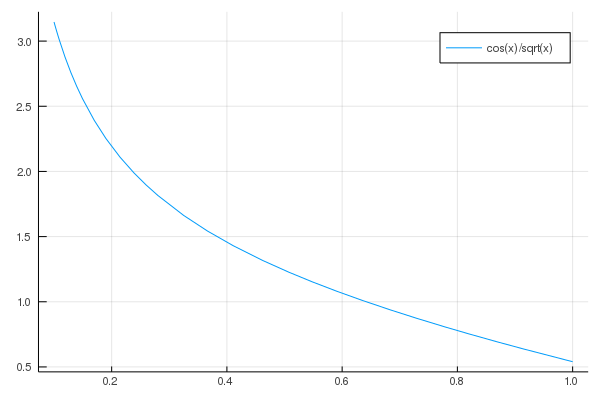
\includegraphics[scale=0.5]{WykresC.png}
    \label{wykresC}
\end{figure}
\begin{figure}[ht]
    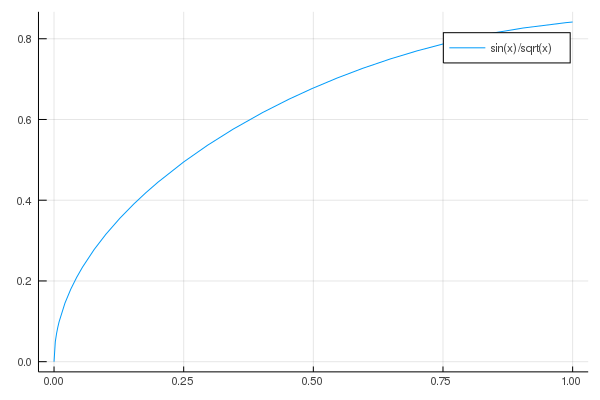
\includegraphics[scale=0.5]{WykresS.png}
    \label{WykresS}
\end{figure}
%\end{figure}
Przyjrzyjmy się wykresom badanych funckji na podanym przedziale. Zauważamy, że $C$ w zerze rozbiega do nieskończoności, a $S$ w zerze zbiega do $0$. Reczywiście obliczenie granic daje wyniki zgodne z wykresami funkcji:
\begin{equation}
\lim_{x\to 0}  \frac{cos(x)}{\sqrt{x}} = \lim_{x\to 0} \frac{cos(0)}{\sqrt{x}} = +\infty
\end{equation}
\begin{equation}
\lim_{x\to 0}  \frac{sin(x)}{\sqrt{x}} = \lim_{x\to 0}  \frac{sin(x)}{x} \sqrt{x} = 0
\end{equation}
Na podstawie tej informacji możemy przypuszczać, że obliczenie całki $I_S$ będzie łatwiejsze niż obliczenie $I_C$, ponieważ $S$ jest ograniczona, a jej wartość w $0$ zgadza się z jej granicą w tym punkcie. $C$ jest nieograniczona i w zerze przyjmuje $0$, ale jej granica w tym punkcie wynosi $+\infty$ zatem obliczenie całki w okolicy $0$ może być niedokładne.\\
Możemy zmienić postać całek $I_C$ i $I_S$ za pomocą podstawienia $x=t^2$ Wtedy:
\begin{equation}
I_C = \int_0^1 \frac{cos(t^2)}{\sqrt{t^2}} 2tdt = \int_0^1 2cos(t^2)
\end{equation}
\begin{equation}
I_S = \int_0^1 \frac{sin(t^2)}{\sqrt{t^2}} 2tdt = \int_0^1 2sin(t^2)
\end{equation}
Otrzymujemy w ten sposób nowe funkcje pod całką $Snew(x) = 2sin(x^2)$ i $Cnew(x) = 2cos(x^2)$. Nowe funkcje mają określone wartości dla wszystkich punktach z przedziału $[0,1]$ i obie funkcjie są ograniczone, więc nie mamy takiego problemu jak przy funkcji $C$.
\begin{figure}[ht]
    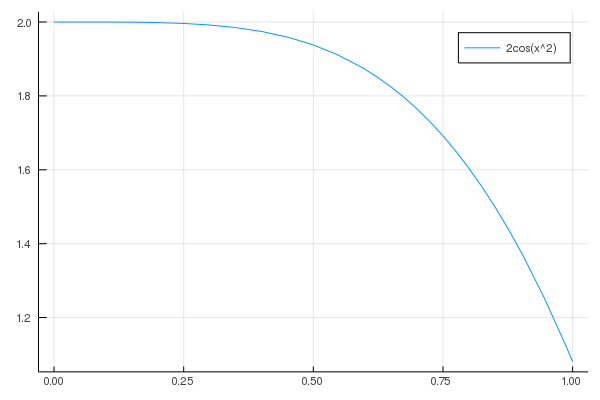
\includegraphics[scale=0.5]{WykresCnew.png}
    \label{wykresCnew}
\end{figure}
\begin{figure}[ht]
    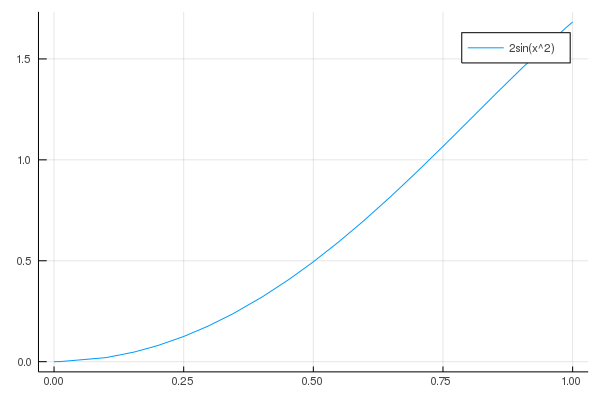
\includegraphics[scale=0.5]{WykresSnew.png}
    \label{WykresSnew}
\end{figure}
\section*{Omówienie wyników}
\dots


\end{document}
